\begin{document}
\maketitle
\begin{abstract}
Activation functions play a crucial role in neural networks because they are the non-linearities which have been attributed to the success story of deep learning. One of the currently most popular activation functions is ReLU, but several competitors have recently been proposed or `discovered', including LReLU functions and \swish. While most works compare newly proposed activation functions on few tasks (usually from image classification) and against few competitors (usually ReLU), we perform the first large-scale comparison of 21 activation functions across eight different NLP tasks. We find that a largely unknown activation function performs most stably across all tasks, the so-called \pentan{} function. We also show that it can successfully replace the \sigmoid{} and \mytanh{} gates in LSTM cells, leading to a 2 percentage point (pp) improvement over the standard choices on a challenging NLP task. 
\end{abstract}

\section{Introduction}

\section{Theory}

\paragraph{Activation functions} 

\begin{table}[!htb]
  \centering
  \begin{tabular}{ll}
  \toprule
    \sigmoid & $f(x)=\sigma(x)=1/(1+\exp(-x))$\\
    %\mytanh & \\
    \swish & $f(x)=x\cdot \sigma(x)$\\
    \maxsig & $f(x)=\max\{x,\sigma(x)\}$\\
    \cosid & $f(x)=\cos(x)-x$\\
    \minsin & $f(x)=\min\{x,\sin(x)\}$\\
    \arctid & $f(x)=\arctan(x)^2-x$\\
    \maxtanh & $f(x)=\max\{x,\tanh(x)\}$\\
    \midrule
    \lrelua & $f(x)=\max\{x,0.01x\}$ \\
    \lrelub & $f(x)=\max\{x,0.3x\}$ \\
    {\small \pentan} & $f(x)=\begin{cases}\tanh(x) & x>0,\\ 0.25\tanh(x) & x\le 0\end{cases}$\\
    \bottomrule
  \end{tabular}
  \caption{Top: \sigmoid{} activation function as well as 6 top performing activation functions from \citet{Ramach:2018}. Bottom: the LReLU functions with different parametrizations as well as \pentan{}.}
  \label{table:functions}
\end{table}

\paragraph{Properties of activation functions} 

\begin{table*}[!htb]
\centering
\footnotesize
\begin{tabular}{llll}
  \toprule
  Property & Description & Problems & Examples \\ \midrule
  derivative & $f'$ & $>1$ exploding gradient (e) &  \sigmoid{} (v), \mytanh{} (v), \cube{} (e)\\
  & & $<1$ vanishing (v) & \\
  zero-centered & range centered around zero? &   if not, slower learning & \mytanh{} ($+$), \relu{} ($-$) \\ 
  saturating & finite limits & vanishing gradient in the limit & \mytanh{}, \pentan{}, \sigmoid{}\\
  monotonicity & $x>y\implies f(x)\ge f(y)$ & unclear & exceptions: \mysin{}, \swish{}, \minsin{} 
  \\ \bottomrule
 \end{tabular}
 \caption{Frequently cited properties of activation functions}.
 \label{table:properties}
\end{table*}

\section{Experiments}\label{sec:experiments}

\subsection{MLP \& Sentence Classification}\label{sec:1}

\paragraph{Model}

\begin{align*}
  \mathbf{x}_i &= f(\mathbf{x}_{i-1}\cdot \mathbf{W}_i+\mathbf{b}_i)\\
  \mathbf{y} &= \text{softmax}(\mathbf{x}_{N}\mathbf{W}_{N+1}+\mathbf{b}_{N+1})
\end{align*}

\paragraph{Approach}

\begin{itemize}[noitemsep,leftmargin=0.6cm]
  \item (1): MR dataset with Sent2Vec-unigram embeddings as input and 1\% of the full data as training data; (2): the same mini-experiment with 50\% of the full data as training data. In both cases, the dev set comprises 10\% of the full data and the rest is for testing. 
  \item (3,4): SUBJ with InferSent embeddings and likewise 1\% and 50\% of the full data as train data, respectively.
  \item (5): The TREC dataset with original split in train and test; 50\% of the train split is used as dev data. 
  \item (6): The AM dataset with original split in train, dev, and test \cite{Eger:2017}, and with InferSent input embeddings. (7): the same mini-experiment with Sent2Vec-unigram embeddings. 
\end{itemize}

\paragraph{Results}

\begin{figure}[htb]
  \centering
  %\scalebox{0.5}{% GNUPLOT: LaTeX picture with Postscript
\begingroup
  \makeatletter
  \providecommand\color[2][]{%
    \GenericError{(gnuplot) \space\space\space\@spaces}{%
      Package color not loaded in conjunction with
      terminal option `colourtext'%
    }{See the gnuplot documentation for explanation.%
    }{Either use 'blacktext' in gnuplot or load the package
      color.sty in LaTeX.}%
    \renewcommand\color[2][]{}%
  }%
  \providecommand\includegraphics[2][]{%
    \GenericError{(gnuplot) \space\space\space\@spaces}{%
      Package graphicx or graphics not loaded%
    }{See the gnuplot documentation for explanation.%
    }{The gnuplot epslatex terminal needs graphicx.sty or graphics.sty.}%
    \renewcommand\includegraphics[2][]{}%
  }%
  \providecommand\rotatebox[2]{#2}%
  \@ifundefined{ifGPcolor}{%
    \newif\ifGPcolor
    \GPcolortrue
  }{}%
  \@ifundefined{ifGPblacktext}{%
    \newif\ifGPblacktext
    \GPblacktexttrue
  }{}%
  % define a \g@addto@macro without @ in the name:
  \let\gplgaddtomacro\g@addto@macro
  % define empty templates for all commands taking text:
  \gdef\gplbacktext{}%
  \gdef\gplfronttext{}%
  \makeatother
  \ifGPblacktext
    % no textcolor at all
    \def\colorrgb#1{}%
    \def\colorgray#1{}%
  \else
    % gray or color?
    \ifGPcolor
      \def\colorrgb#1{\color[rgb]{#1}}%
      \def\colorgray#1{\color[gray]{#1}}%
      \expandafter\def\csname LTw\endcsname{\color{white}}%
      \expandafter\def\csname LTb\endcsname{\color{black}}%
      \expandafter\def\csname LTa\endcsname{\color{black}}%
      \expandafter\def\csname LT0\endcsname{\color[rgb]{1,0,0}}%
      \expandafter\def\csname LT1\endcsname{\color[rgb]{0,1,0}}%
      \expandafter\def\csname LT2\endcsname{\color[rgb]{0,0,1}}%
      \expandafter\def\csname LT3\endcsname{\color[rgb]{1,0,1}}%
      \expandafter\def\csname LT4\endcsname{\color[rgb]{0,1,1}}%
      \expandafter\def\csname LT5\endcsname{\color[rgb]{1,1,0}}%
      \expandafter\def\csname LT6\endcsname{\color[rgb]{0,0,0}}%
      \expandafter\def\csname LT7\endcsname{\color[rgb]{1,0.3,0}}%
      \expandafter\def\csname LT8\endcsname{\color[rgb]{0.5,0.5,0.5}}%
    \else
      % gray
      \def\colorrgb#1{\color{black}}%
      \def\colorgray#1{\color[gray]{#1}}%
      \expandafter\def\csname LTw\endcsname{\color{white}}%
      \expandafter\def\csname LTb\endcsname{\color{black}}%
      \expandafter\def\csname LTa\endcsname{\color{black}}%
      \expandafter\def\csname LT0\endcsname{\color{black}}%
      \expandafter\def\csname LT1\endcsname{\color{black}}%
      \expandafter\def\csname LT2\endcsname{\color{black}}%
      \expandafter\def\csname LT3\endcsname{\color{black}}%
      \expandafter\def\csname LT4\endcsname{\color{black}}%
      \expandafter\def\csname LT5\endcsname{\color{black}}%
      \expandafter\def\csname LT6\endcsname{\color{black}}%
      \expandafter\def\csname LT7\endcsname{\color{black}}%
      \expandafter\def\csname LT8\endcsname{\color{black}}%
    \fi
  \fi
  \setlength{\unitlength}{0.0500bp}%
  \begin{picture}(8502.00,6802.00)%
    \gplgaddtomacro\gplbacktext{%
      \csname LTb\endcsname%
      \put(784,1711){\makebox(0,0)[r]{\strut{} 75.2}}%
      \csname LTb\endcsname%
      \put(784,2156){\makebox(0,0)[r]{\strut{} 75.3}}%
      \csname LTb\endcsname%
      \put(784,2602){\makebox(0,0)[r]{\strut{} 75.4}}%
      \csname LTb\endcsname%
      \put(784,3047){\makebox(0,0)[r]{\strut{} 75.5}}%
      \csname LTb\endcsname%
      \put(784,3492){\makebox(0,0)[r]{\strut{} 75.6}}%
      \csname LTb\endcsname%
      \put(784,3937){\makebox(0,0)[r]{\strut{} 75.7}}%
      \csname LTb\endcsname%
      \put(784,4383){\makebox(0,0)[r]{\strut{} 75.8}}%
      \csname LTb\endcsname%
      \put(784,4828){\makebox(0,0)[r]{\strut{} 75.9}}%
      \csname LTb\endcsname%
      \put(784,5273){\makebox(0,0)[r]{\strut{} 76}}%
      \csname LTb\endcsname%
      \put(784,5718){\makebox(0,0)[r]{\strut{} 76.1}}%
      \csname LTb\endcsname%
      \put(784,6164){\makebox(0,0)[r]{\strut{} 76.2}}%
      \csname LTb\endcsname%
      \put(784,6609){\makebox(0,0)[r]{\strut{} 76.3}}%
      \csname LTb\endcsname%
      \put(880,1408){\rotatebox{-270}{\makebox(0,0)[r]{\strut{}\relu}}}%
      \csname LTb\endcsname%
      \put(1223,1408){\rotatebox{-270}{\makebox(0,0)[r]{\strut{}maxout-4}}}%
      \csname LTb\endcsname%
      \put(1565,1408){\rotatebox{-270}{\makebox(0,0)[r]{\strut{}leakyrelu-0.01}}}%
      \csname LTb\endcsname%
      \put(1908,1408){\rotatebox{-270}{\makebox(0,0)[r]{\strut{}maxout-3}}}%
      \csname LTb\endcsname%
      \put(2251,1408){\rotatebox{-270}{\makebox(0,0)[r]{\strut{}\pentan}}}%
      \csname LTb\endcsname%
      \put(2593,1408){\rotatebox{-270}{\makebox(0,0)[r]{\strut{}maxout-2}}}%
      \csname LTb\endcsname%
      \put(2936,1408){\rotatebox{-270}{\makebox(0,0)[r]{\strut{}\prelu}}}%
      \csname LTb\endcsname%
      \put(3279,1408){\rotatebox{-270}{\makebox(0,0)[r]{\strut{}\minsin}}}%
      \csname LTb\endcsname%
      \put(3621,1408){\rotatebox{-270}{\makebox(0,0)[r]{\strut{}\swish}}}%
      \csname LTb\endcsname%
      \put(3964,1408){\rotatebox{-270}{\makebox(0,0)[r]{\strut{}\mytanh}}}%
      \csname LTb\endcsname%
      \put(4307,1408){\rotatebox{-270}{\makebox(0,0)[r]{\strut{}\selu}}}%
      \csname LTb\endcsname%
      \put(4649,1408){\rotatebox{-270}{\makebox(0,0)[r]{\strut{}\mysin}}}%
      \csname LTb\endcsname%
      \put(4992,1408){\rotatebox{-270}{\makebox(0,0)[r]{\strut{}leakyrelu-0.3}}}%
      \csname LTb\endcsname%
      \put(5334,1408){\rotatebox{-270}{\makebox(0,0)[r]{\strut{}\maxtanh}}}%
      \csname LTb\endcsname%
      \put(5677,1408){\rotatebox{-270}{\makebox(0,0)[r]{\strut{}\maxsig}}}%
      \csname LTb\endcsname%
      \put(6020,1408){\rotatebox{-270}{\makebox(0,0)[r]{\strut{}\sigmoid}}}%
      \csname LTb\endcsname%
      \put(6362,1408){\rotatebox{-270}{\makebox(0,0)[r]{\strut{}\cosid}}}%
      \csname LTb\endcsname%
      \put(6705,1408){\rotatebox{-270}{\makebox(0,0)[r]{\strut{}\arctid}}}%
      \csname LTb\endcsname%
      \put(7048,1408){\rotatebox{-270}{\makebox(0,0)[r]{\strut{}\cube}}}%
      \csname LTb\endcsname%
      \put(7390,1408){\rotatebox{-270}{\makebox(0,0)[r]{\strut{}\elu}}}%
      \csname LTb\endcsname%
      \put(7733,1408){\rotatebox{-270}{\makebox(0,0)[r]{\strut{}\linear}}}%
      \put(7829,2261){\makebox(0,0)[l]{\strut{} 50}}%
      \put(7829,3348){\makebox(0,0)[l]{\strut{} 55}}%
      \put(7829,4435){\makebox(0,0)[l]{\strut{} 60}}%
      \put(7829,5522){\makebox(0,0)[l]{\strut{} 65}}%
      \put(7829,6609){\makebox(0,0)[l]{\strut{} 70}}%
      \put(128,4056){\rotatebox{-270}{\makebox(0,0){\strut{}Score}}}%
    }%
    \gplgaddtomacro\gplfronttext{%
      \csname LTb\endcsname%
      \put(6998,6466){\makebox(0,0)[r]{\strut{}Best}}%
      \csname LTb\endcsname%
      \put(6998,6306){\makebox(0,0)[r]{\strut{}Avg}}%
    }%
    \gplbacktext
    \put(0,0){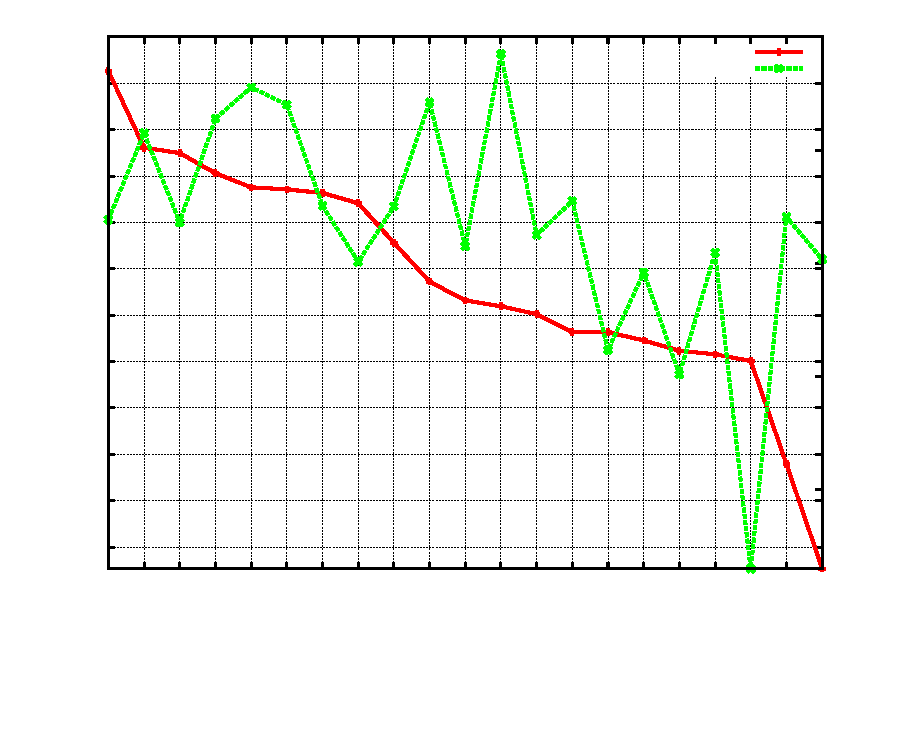
\includegraphics{plots/sent3}}%
    \gplfronttext
  \end{picture}%
\endgroup
}
  \scalebox{0.5}{% GNUPLOT: LaTeX picture with Postscript
\begingroup
  \makeatletter
  \providecommand\color[2][]{%
    \GenericError{(gnuplot) \space\space\space\@spaces}{%
      Package color not loaded in conjunction with
      terminal option `colourtext'%
    }{See the gnuplot documentation for explanation.%
    }{Either use 'blacktext' in gnuplot or load the package
      color.sty in LaTeX.}%
    \renewcommand\color[2][]{}%
  }%
  \providecommand\includegraphics[2][]{%
    \GenericError{(gnuplot) \space\space\space\@spaces}{%
      Package graphicx or graphics not loaded%
    }{See the gnuplot documentation for explanation.%
    }{The gnuplot epslatex terminal needs graphicx.sty or graphics.sty.}%
    \renewcommand\includegraphics[2][]{}%
  }%
  \providecommand\rotatebox[2]{#2}%
  \@ifundefined{ifGPcolor}{%
    \newif\ifGPcolor
    \GPcolortrue
  }{}%
  \@ifundefined{ifGPblacktext}{%
    \newif\ifGPblacktext
    \GPblacktexttrue
  }{}%
  % define a \g@addto@macro without @ in the name:
  \let\gplgaddtomacro\g@addto@macro
  % define empty templates for all commands taking text:
  \gdef\gplbacktext{}%
  \gdef\gplfronttext{}%
  \makeatother
  \ifGPblacktext
    % no textcolor at all
    \def\colorrgb#1{}%
    \def\colorgray#1{}%
  \else
    % gray or color?
    \ifGPcolor
      \def\colorrgb#1{\color[rgb]{#1}}%
      \def\colorgray#1{\color[gray]{#1}}%
      \expandafter\def\csname LTw\endcsname{\color{white}}%
      \expandafter\def\csname LTb\endcsname{\color{black}}%
      \expandafter\def\csname LTa\endcsname{\color{black}}%
      \expandafter\def\csname LT0\endcsname{\color[rgb]{1,0,0}}%
      \expandafter\def\csname LT1\endcsname{\color[rgb]{0,1,0}}%
      \expandafter\def\csname LT2\endcsname{\color[rgb]{0,0,1}}%
      \expandafter\def\csname LT3\endcsname{\color[rgb]{1,0,1}}%
      \expandafter\def\csname LT4\endcsname{\color[rgb]{0,1,1}}%
      \expandafter\def\csname LT5\endcsname{\color[rgb]{1,1,0}}%
      \expandafter\def\csname LT6\endcsname{\color[rgb]{0,0,0}}%
      \expandafter\def\csname LT7\endcsname{\color[rgb]{1,0.3,0}}%
      \expandafter\def\csname LT8\endcsname{\color[rgb]{0.5,0.5,0.5}}%
    \else
      % gray
      \def\colorrgb#1{\color{black}}%
      \def\colorgray#1{\color[gray]{#1}}%
      \expandafter\def\csname LTw\endcsname{\color{white}}%
      \expandafter\def\csname LTb\endcsname{\color{black}}%
      \expandafter\def\csname LTa\endcsname{\color{black}}%
      \expandafter\def\csname LT0\endcsname{\color{black}}%
      \expandafter\def\csname LT1\endcsname{\color{black}}%
      \expandafter\def\csname LT2\endcsname{\color{black}}%
      \expandafter\def\csname LT3\endcsname{\color{black}}%
      \expandafter\def\csname LT4\endcsname{\color{black}}%
      \expandafter\def\csname LT5\endcsname{\color{black}}%
      \expandafter\def\csname LT6\endcsname{\color{black}}%
      \expandafter\def\csname LT7\endcsname{\color{black}}%
      \expandafter\def\csname LT8\endcsname{\color{black}}%
    \fi
  \fi
  \setlength{\unitlength}{0.0500bp}%
  \begin{picture}(8502.00,6802.00)%
    \gplgaddtomacro\gplbacktext{%
      \csname LTb\endcsname%
      \put(784,2001){\makebox(0,0)[r]{\strut{} 98}}%
      \csname LTb\endcsname%
      \put(784,3153){\makebox(0,0)[r]{\strut{} 98.5}}%
      \csname LTb\endcsname%
      \put(784,4305){\makebox(0,0)[r]{\strut{} 99}}%
      \csname LTb\endcsname%
      \put(784,5457){\makebox(0,0)[r]{\strut{} 99.5}}%
      \csname LTb\endcsname%
      \put(784,6609){\makebox(0,0)[r]{\strut{} 100}}%
      \csname LTb\endcsname%
      \put(880,1408){\rotatebox{-270}{\makebox(0,0)[r]{\strut{}\relu}}}%
      \csname LTb\endcsname%
      \put(1223,1408){\rotatebox{-270}{\makebox(0,0)[r]{\strut{}\lrelua}}}%
      \csname LTb\endcsname%
      \put(1565,1408){\rotatebox{-270}{\makebox(0,0)[r]{\strut{}\maxoutc}}}%
      \csname LTb\endcsname%
      \put(1908,1408){\rotatebox{-270}{\makebox(0,0)[r]{\strut{}\maxoutb}}}%
      \csname LTb\endcsname%
      \put(2251,1408){\rotatebox{-270}{\makebox(0,0)[r]{\strut{}\pentan}}}%
      \csname LTb\endcsname%
      \put(2593,1408){\rotatebox{-270}{\makebox(0,0)[r]{\strut{}\prelu}}}%
      \csname LTb\endcsname%
      \put(2936,1408){\rotatebox{-270}{\makebox(0,0)[r]{\strut{}\maxouta}}}%
      \csname LTb\endcsname%
      \put(3279,1408){\rotatebox{-270}{\makebox(0,0)[r]{\strut{}\minsin}}}%
      \csname LTb\endcsname%
      \put(3621,1408){\rotatebox{-270}{\makebox(0,0)[r]{\strut{}\swish}}}%
      \csname LTb\endcsname%
      \put(3964,1408){\rotatebox{-270}{\makebox(0,0)[r]{\strut{}\mytanh}}}%
      \csname LTb\endcsname%
      \put(4307,1408){\rotatebox{-270}{\makebox(0,0)[r]{\strut{}\selu}}}%
      \csname LTb\endcsname%
      \put(4649,1408){\rotatebox{-270}{\makebox(0,0)[r]{\strut{}\mysin}}}%
      \csname LTb\endcsname%
      \put(4992,1408){\rotatebox{-270}{\makebox(0,0)[r]{\strut{}\lrelub}}}%
      \csname LTb\endcsname%
      \put(5334,1408){\rotatebox{-270}{\makebox(0,0)[r]{\strut{}\maxsig}}}%
      \csname LTb\endcsname%
      \put(5677,1408){\rotatebox{-270}{\makebox(0,0)[r]{\strut{}\maxtanh}}}%
      \csname LTb\endcsname%
      \put(6020,1408){\rotatebox{-270}{\makebox(0,0)[r]{\strut{}\cosid}}}%
      \csname LTb\endcsname%
      \put(6362,1408){\rotatebox{-270}{\makebox(0,0)[r]{\strut{}\cube}}}%
      \csname LTb\endcsname%
      \put(6705,1408){\rotatebox{-270}{\makebox(0,0)[r]{\strut{}\sigmoid}}}%
      \csname LTb\endcsname%
      \put(7048,1408){\rotatebox{-270}{\makebox(0,0)[r]{\strut{}\arctid}}}%
      \csname LTb\endcsname%
      \put(7390,1408){\rotatebox{-270}{\makebox(0,0)[r]{\strut{}\elu}}}%
      \csname LTb\endcsname%
      \put(7733,1408){\rotatebox{-270}{\makebox(0,0)[r]{\strut{}\linear}}}%
      \put(7829,2103){\makebox(0,0)[l]{\strut{} 69}}%
      \put(7829,2830){\makebox(0,0)[l]{\strut{} 74}}%
      \put(7829,3557){\makebox(0,0)[l]{\strut{} 79}}%
      \put(7829,4284){\makebox(0,0)[l]{\strut{} 84}}%
      \put(7829,5010){\makebox(0,0)[l]{\strut{} 89}}%
      \put(7829,5737){\makebox(0,0)[l]{\strut{} 94}}%
      \put(7829,6464){\makebox(0,0)[l]{\strut{} 99}}%
      \put(128,4056){\rotatebox{-270}{\makebox(0,0){\strut{}Score}}}%
    }%
    \gplgaddtomacro\gplfronttext{%
      \csname LTb\endcsname%
      \put(6998,6466){\makebox(0,0)[r]{\strut{}\best{}}}%
      \csname LTb\endcsname%
      \put(6998,6306){\makebox(0,0)[r]{\strut{}\avg{}}}%
    }%
    \gplbacktext
    \put(0,0){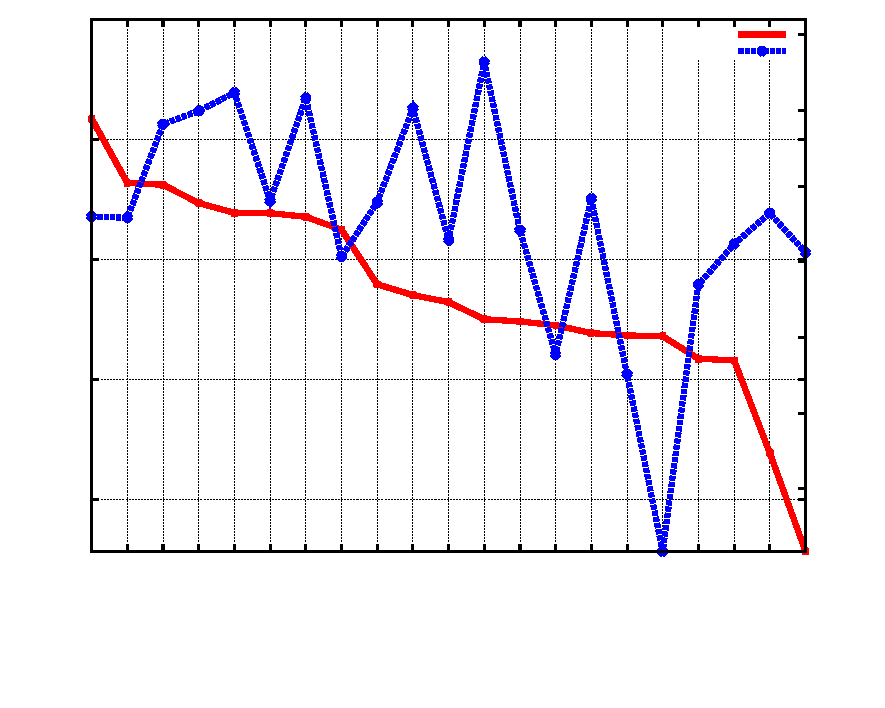
\includegraphics{plots/sent-X.pdf}}%
    \gplfronttext
  \end{picture}%
\endgroup
}
  \caption{Sentence Classification. Left y-axis: \best. Right y-axis: \avg{}. Score on y-axes is the average over all mini-experiments.}
  \label{fig:sent}
\end{figure}

\subsection{CNN \& Document Classification}

\paragraph{Model}

\begin{align*}
  c_i = f(\mathbf{w}\cdot \mathbf{x}_{i:i+h-1}+b).
\end{align*}

\paragraph{Approach}

\begin{itemize}[noitemsep,leftmargin=0.6cm]
\item (1,2) NG dataset with 5\% and 50\%, respectively of the full data as train data. In both cases, 10\% of the full data is used as dev data, and the rest as test data.  
\item (3,4) Same as (1,2) for R8. 
%R8 dataset with same specifications as for NG.
\end{itemize}

\paragraph{Results}

\begin{figure}[!htb]
\centering
%\scalebox{0.5}{% GNUPLOT: LaTeX picture with Postscript
\begingroup
  \makeatletter
  \providecommand\color[2][]{%
    \GenericError{(gnuplot) \space\space\space\@spaces}{%
      Package color not loaded in conjunction with
      terminal option `colourtext'%
    }{See the gnuplot documentation for explanation.%
    }{Either use 'blacktext' in gnuplot or load the package
      color.sty in LaTeX.}%
    \renewcommand\color[2][]{}%
  }%
  \providecommand\includegraphics[2][]{%
    \GenericError{(gnuplot) \space\space\space\@spaces}{%
      Package graphicx or graphics not loaded%
    }{See the gnuplot documentation for explanation.%
    }{The gnuplot epslatex terminal needs graphicx.sty or graphics.sty.}%
    \renewcommand\includegraphics[2][]{}%
  }%
  \providecommand\rotatebox[2]{#2}%
  \@ifundefined{ifGPcolor}{%
    \newif\ifGPcolor
    \GPcolortrue
  }{}%
  \@ifundefined{ifGPblacktext}{%
    \newif\ifGPblacktext
    \GPblacktexttrue
  }{}%
  % define a \g@addto@macro without @ in the name:
  \let\gplgaddtomacro\g@addto@macro
  % define empty templates for all commands taking text:
  \gdef\gplbacktext{}%
  \gdef\gplfronttext{}%
  \makeatother
  \ifGPblacktext
    % no textcolor at all
    \def\colorrgb#1{}%
    \def\colorgray#1{}%
  \else
    % gray or color?
    \ifGPcolor
      \def\colorrgb#1{\color[rgb]{#1}}%
      \def\colorgray#1{\color[gray]{#1}}%
      \expandafter\def\csname LTw\endcsname{\color{white}}%
      \expandafter\def\csname LTb\endcsname{\color{black}}%
      \expandafter\def\csname LTa\endcsname{\color{black}}%
      \expandafter\def\csname LT0\endcsname{\color[rgb]{1,0,0}}%
      \expandafter\def\csname LT1\endcsname{\color[rgb]{0,1,0}}%
      \expandafter\def\csname LT2\endcsname{\color[rgb]{0,0,1}}%
      \expandafter\def\csname LT3\endcsname{\color[rgb]{1,0,1}}%
      \expandafter\def\csname LT4\endcsname{\color[rgb]{0,1,1}}%
      \expandafter\def\csname LT5\endcsname{\color[rgb]{1,1,0}}%
      \expandafter\def\csname LT6\endcsname{\color[rgb]{0,0,0}}%
      \expandafter\def\csname LT7\endcsname{\color[rgb]{1,0.3,0}}%
      \expandafter\def\csname LT8\endcsname{\color[rgb]{0.5,0.5,0.5}}%
    \else
      % gray
      \def\colorrgb#1{\color{black}}%
      \def\colorgray#1{\color[gray]{#1}}%
      \expandafter\def\csname LTw\endcsname{\color{white}}%
      \expandafter\def\csname LTb\endcsname{\color{black}}%
      \expandafter\def\csname LTa\endcsname{\color{black}}%
      \expandafter\def\csname LT0\endcsname{\color{black}}%
      \expandafter\def\csname LT1\endcsname{\color{black}}%
      \expandafter\def\csname LT2\endcsname{\color{black}}%
      \expandafter\def\csname LT3\endcsname{\color{black}}%
      \expandafter\def\csname LT4\endcsname{\color{black}}%
      \expandafter\def\csname LT5\endcsname{\color{black}}%
      \expandafter\def\csname LT6\endcsname{\color{black}}%
      \expandafter\def\csname LT7\endcsname{\color{black}}%
      \expandafter\def\csname LT8\endcsname{\color{black}}%
    \fi
  \fi
  \setlength{\unitlength}{0.0500bp}%
  \begin{picture}(8502.00,6802.00)%
    \gplgaddtomacro\gplbacktext{%
      \csname LTb\endcsname%
      \put(784,1687){\makebox(0,0)[r]{\strut{} 79}}%
      \csname LTb\endcsname%
      \put(784,1960){\makebox(0,0)[r]{\strut{} 79.2}}%
      \csname LTb\endcsname%
      \put(784,2234){\makebox(0,0)[r]{\strut{} 79.4}}%
      \csname LTb\endcsname%
      \put(784,2507){\makebox(0,0)[r]{\strut{} 79.6}}%
      \csname LTb\endcsname%
      \put(784,2781){\makebox(0,0)[r]{\strut{} 79.8}}%
      \csname LTb\endcsname%
      \put(784,3054){\makebox(0,0)[r]{\strut{} 80}}%
      \csname LTb\endcsname%
      \put(784,3328){\makebox(0,0)[r]{\strut{} 80.2}}%
      \csname LTb\endcsname%
      \put(784,3601){\makebox(0,0)[r]{\strut{} 80.4}}%
      \csname LTb\endcsname%
      \put(784,3875){\makebox(0,0)[r]{\strut{} 80.6}}%
      \csname LTb\endcsname%
      \put(784,4148){\makebox(0,0)[r]{\strut{} 80.8}}%
      \csname LTb\endcsname%
      \put(784,4421){\makebox(0,0)[r]{\strut{} 81}}%
      \csname LTb\endcsname%
      \put(784,4695){\makebox(0,0)[r]{\strut{} 81.2}}%
      \csname LTb\endcsname%
      \put(784,4968){\makebox(0,0)[r]{\strut{} 81.4}}%
      \csname LTb\endcsname%
      \put(784,5242){\makebox(0,0)[r]{\strut{} 81.6}}%
      \csname LTb\endcsname%
      \put(784,5515){\makebox(0,0)[r]{\strut{} 81.8}}%
      \csname LTb\endcsname%
      \put(784,5789){\makebox(0,0)[r]{\strut{} 82}}%
      \csname LTb\endcsname%
      \put(784,6062){\makebox(0,0)[r]{\strut{} 82.2}}%
      \csname LTb\endcsname%
      \put(784,6336){\makebox(0,0)[r]{\strut{} 82.4}}%
      \csname LTb\endcsname%
      \put(784,6609){\makebox(0,0)[r]{\strut{} 82.6}}%
      \csname LTb\endcsname%
      \put(880,1408){\rotatebox{-270}{\makebox(0,0)[r]{\strut{}elu}}}%
      \csname LTb\endcsname%
      \put(1223,1408){\rotatebox{-270}{\makebox(0,0)[r]{\strut{}selu}}}%
      \csname LTb\endcsname%
      \put(1565,1408){\rotatebox{-270}{\makebox(0,0)[r]{\strut{}tanh}}}%
      \csname LTb\endcsname%
      \put(1908,1408){\rotatebox{-270}{\makebox(0,0)[r]{\strut{}minsin}}}%
      \csname LTb\endcsname%
      \put(2251,1408){\rotatebox{-270}{\makebox(0,0)[r]{\strut{}maxout-2}}}%
      \csname LTb\endcsname%
      \put(2593,1408){\rotatebox{-270}{\makebox(0,0)[r]{\strut{}penalized\_tanh}}}%
      \csname LTb\endcsname%
      \put(2936,1408){\rotatebox{-270}{\makebox(0,0)[r]{\strut{}maxout-3}}}%
      \csname LTb\endcsname%
      \put(3279,1408){\rotatebox{-270}{\makebox(0,0)[r]{\strut{}sin}}}%
      \csname LTb\endcsname%
      \put(3621,1408){\rotatebox{-270}{\makebox(0,0)[r]{\strut{}maxout-4}}}%
      \csname LTb\endcsname%
      \put(3964,1408){\rotatebox{-270}{\makebox(0,0)[r]{\strut{}prelu}}}%
      \csname LTb\endcsname%
      \put(4307,1408){\rotatebox{-270}{\makebox(0,0)[r]{\strut{}leakyrelu-0.3}}}%
      \csname LTb\endcsname%
      \put(4649,1408){\rotatebox{-270}{\makebox(0,0)[r]{\strut{}linear}}}%
      \csname LTb\endcsname%
      \put(4992,1408){\rotatebox{-270}{\makebox(0,0)[r]{\strut{}maxtanh}}}%
      \csname LTb\endcsname%
      \put(5334,1408){\rotatebox{-270}{\makebox(0,0)[r]{\strut{}leakyrelu-0.01}}}%
      \csname LTb\endcsname%
      \put(5677,1408){\rotatebox{-270}{\makebox(0,0)[r]{\strut{}relu}}}%
      \csname LTb\endcsname%
      \put(6020,1408){\rotatebox{-270}{\makebox(0,0)[r]{\strut{}tanhrev}}}%
      \csname LTb\endcsname%
      \put(6362,1408){\rotatebox{-270}{\makebox(0,0)[r]{\strut{}swish}}}%
      \csname LTb\endcsname%
      \put(6705,1408){\rotatebox{-270}{\makebox(0,0)[r]{\strut{}cosper}}}%
      \csname LTb\endcsname%
      \put(7048,1408){\rotatebox{-270}{\makebox(0,0)[r]{\strut{}sigmoid}}}%
      \csname LTb\endcsname%
      \put(7390,1408){\rotatebox{-270}{\makebox(0,0)[r]{\strut{}maxsig}}}%
      \csname LTb\endcsname%
      \put(7733,1408){\rotatebox{-270}{\makebox(0,0)[r]{\strut{}cube}}}%
      \put(7829,2171){\makebox(0,0)[l]{\strut{} 45}}%
      \put(7829,3059){\makebox(0,0)[l]{\strut{} 50}}%
      \put(7829,3946){\makebox(0,0)[l]{\strut{} 55}}%
      \put(7829,4834){\makebox(0,0)[l]{\strut{} 60}}%
      \put(7829,5721){\makebox(0,0)[l]{\strut{} 65}}%
      \put(7829,6609){\makebox(0,0)[l]{\strut{} 70}}%
      \csname LTb\endcsname%
      \put(128,4056){\rotatebox{-270}{\makebox(0,0){\strut{}Score}}}%
    }%
    \gplgaddtomacro\gplfronttext{%
      \csname LTb\endcsname%
      \put(6998,1807){\makebox(0,0)[r]{\strut{}Best}}%
      \csname LTb\endcsname%
      \put(6998,1647){\makebox(0,0)[r]{\strut{}Avg}}%
    }%
    \gplbacktext
    \put(0,0){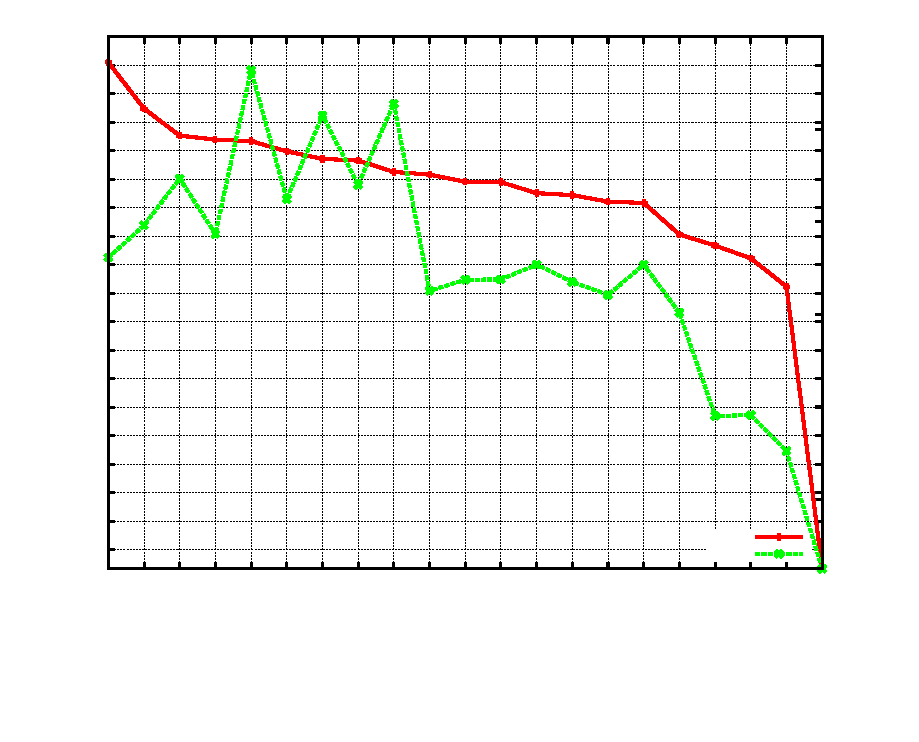
\includegraphics{plots/doc2}}%
    \gplfronttext
  \end{picture}%
\endgroup
}
\scalebox{0.5}{% GNUPLOT: LaTeX picture with Postscript
\begingroup
  \makeatletter
  \providecommand\color[2][]{%
    \GenericError{(gnuplot) \space\space\space\@spaces}{%
      Package color not loaded in conjunction with
      terminal option `colourtext'%
    }{See the gnuplot documentation for explanation.%
    }{Either use 'blacktext' in gnuplot or load the package
      color.sty in LaTeX.}%
    \renewcommand\color[2][]{}%
  }%
  \providecommand\includegraphics[2][]{%
    \GenericError{(gnuplot) \space\space\space\@spaces}{%
      Package graphicx or graphics not loaded%
    }{See the gnuplot documentation for explanation.%
    }{The gnuplot epslatex terminal needs graphicx.sty or graphics.sty.}%
    \renewcommand\includegraphics[2][]{}%
  }%
  \providecommand\rotatebox[2]{#2}%
  \@ifundefined{ifGPcolor}{%
    \newif\ifGPcolor
    \GPcolortrue
  }{}%
  \@ifundefined{ifGPblacktext}{%
    \newif\ifGPblacktext
    \GPblacktexttrue
  }{}%
  % define a \g@addto@macro without @ in the name:
  \let\gplgaddtomacro\g@addto@macro
  % define empty templates for all commands taking text:
  \gdef\gplbacktext{}%
  \gdef\gplfronttext{}%
  \makeatother
  \ifGPblacktext
    % no textcolor at all
    \def\colorrgb#1{}%
    \def\colorgray#1{}%
  \else
    % gray or color?
    \ifGPcolor
      \def\colorrgb#1{\color[rgb]{#1}}%
      \def\colorgray#1{\color[gray]{#1}}%
      \expandafter\def\csname LTw\endcsname{\color{white}}%
      \expandafter\def\csname LTb\endcsname{\color{black}}%
      \expandafter\def\csname LTa\endcsname{\color{black}}%
      \expandafter\def\csname LT0\endcsname{\color[rgb]{1,0,0}}%
      \expandafter\def\csname LT1\endcsname{\color[rgb]{0,1,0}}%
      \expandafter\def\csname LT2\endcsname{\color[rgb]{0,0,1}}%
      \expandafter\def\csname LT3\endcsname{\color[rgb]{1,0,1}}%
      \expandafter\def\csname LT4\endcsname{\color[rgb]{0,1,1}}%
      \expandafter\def\csname LT5\endcsname{\color[rgb]{1,1,0}}%
      \expandafter\def\csname LT6\endcsname{\color[rgb]{0,0,0}}%
      \expandafter\def\csname LT7\endcsname{\color[rgb]{1,0.3,0}}%
      \expandafter\def\csname LT8\endcsname{\color[rgb]{0.5,0.5,0.5}}%
    \else
      % gray
      \def\colorrgb#1{\color{black}}%
      \def\colorgray#1{\color[gray]{#1}}%
      \expandafter\def\csname LTw\endcsname{\color{white}}%
      \expandafter\def\csname LTb\endcsname{\color{black}}%
      \expandafter\def\csname LTa\endcsname{\color{black}}%
      \expandafter\def\csname LT0\endcsname{\color{black}}%
      \expandafter\def\csname LT1\endcsname{\color{black}}%
      \expandafter\def\csname LT2\endcsname{\color{black}}%
      \expandafter\def\csname LT3\endcsname{\color{black}}%
      \expandafter\def\csname LT4\endcsname{\color{black}}%
      \expandafter\def\csname LT5\endcsname{\color{black}}%
      \expandafter\def\csname LT6\endcsname{\color{black}}%
      \expandafter\def\csname LT7\endcsname{\color{black}}%
      \expandafter\def\csname LT8\endcsname{\color{black}}%
    \fi
  \fi
  \setlength{\unitlength}{0.0500bp}%
  \begin{picture}(8502.00,6802.00)%
    \gplgaddtomacro\gplbacktext{%
      \csname LTb\endcsname%
      \put(784,1551){\makebox(0,0)[r]{\strut{} 94.5}}%
      \csname LTb\endcsname%
      \put(784,2010){\makebox(0,0)[r]{\strut{} 95}}%
      \csname LTb\endcsname%
      \put(784,2470){\makebox(0,0)[r]{\strut{} 95.5}}%
      \csname LTb\endcsname%
      \put(784,2930){\makebox(0,0)[r]{\strut{} 96}}%
      \csname LTb\endcsname%
      \put(784,3390){\makebox(0,0)[r]{\strut{} 96.5}}%
      \csname LTb\endcsname%
      \put(784,3850){\makebox(0,0)[r]{\strut{} 97}}%
      \csname LTb\endcsname%
      \put(784,4310){\makebox(0,0)[r]{\strut{} 97.5}}%
      \csname LTb\endcsname%
      \put(784,4770){\makebox(0,0)[r]{\strut{} 98}}%
      \csname LTb\endcsname%
      \put(784,5229){\makebox(0,0)[r]{\strut{} 98.5}}%
      \csname LTb\endcsname%
      \put(784,5689){\makebox(0,0)[r]{\strut{} 99}}%
      \csname LTb\endcsname%
      \put(784,6149){\makebox(0,0)[r]{\strut{} 99.5}}%
      \csname LTb\endcsname%
      \put(784,6609){\makebox(0,0)[r]{\strut{} 100}}%
      \csname LTb\endcsname%
      \put(880,1408){\rotatebox{-270}{\makebox(0,0)[r]{\strut{}\elu}}}%
      \csname LTb\endcsname%
      \put(1218,1408){\rotatebox{-270}{\makebox(0,0)[r]{\strut{}\selu}}}%
      \csname LTb\endcsname%
      \put(1556,1408){\rotatebox{-270}{\makebox(0,0)[r]{\strut{}\maxouta}}}%
      \csname LTb\endcsname%
      \put(1894,1408){\rotatebox{-270}{\makebox(0,0)[r]{\strut{}\mytanh}}}%
      \csname LTb\endcsname%
      \put(2231,1408){\rotatebox{-270}{\makebox(0,0)[r]{\strut{}\minsin}}}%
      \csname LTb\endcsname%
      \put(2569,1408){\rotatebox{-270}{\makebox(0,0)[r]{\strut{}\pentan}}}%
      \csname LTb\endcsname%
      \put(2907,1408){\rotatebox{-270}{\makebox(0,0)[r]{\strut{}\maxoutb}}}%
      \csname LTb\endcsname%
      \put(3245,1408){\rotatebox{-270}{\makebox(0,0)[r]{\strut{}\mysin}}}%
      \csname LTb\endcsname%
      \put(3583,1408){\rotatebox{-270}{\makebox(0,0)[r]{\strut{}\maxoutc}}}%
      \csname LTb\endcsname%
      \put(3921,1408){\rotatebox{-270}{\makebox(0,0)[r]{\strut{}\prelu}}}%
      \csname LTb\endcsname%
      \put(4259,1408){\rotatebox{-270}{\makebox(0,0)[r]{\strut{}\linear}}}%
      \csname LTb\endcsname%
      \put(4596,1408){\rotatebox{-270}{\makebox(0,0)[r]{\strut{}\lrelub}}}%
      \csname LTb\endcsname%
      \put(4934,1408){\rotatebox{-270}{\makebox(0,0)[r]{\strut{}\maxtanh}}}%
      \csname LTb\endcsname%
      \put(5272,1408){\rotatebox{-270}{\makebox(0,0)[r]{\strut{}\lrelua}}}%
      \csname LTb\endcsname%
      \put(5610,1408){\rotatebox{-270}{\makebox(0,0)[r]{\strut{}\relu}}}%
      \csname LTb\endcsname%
      \put(5948,1408){\rotatebox{-270}{\makebox(0,0)[r]{\strut{}\arctid}}}%
      \csname LTb\endcsname%
      \put(6286,1408){\rotatebox{-270}{\makebox(0,0)[r]{\strut{}\cosid}}}%
      \csname LTb\endcsname%
      \put(6623,1408){\rotatebox{-270}{\makebox(0,0)[r]{\strut{}\sigmoid}}}%
      \csname LTb\endcsname%
      \put(6961,1408){\rotatebox{-270}{\makebox(0,0)[r]{\strut{}\swish}}}%
      \csname LTb\endcsname%
      \put(7299,1408){\rotatebox{-270}{\makebox(0,0)[r]{\strut{}\maxsig}}}%
      \csname LTb\endcsname%
      \put(7637,1408){\rotatebox{-270}{\makebox(0,0)[r]{\strut{}\cube}}}%
      \put(7733,1992){\makebox(0,0)[l]{\strut{} 60}}%
      \put(7733,2569){\makebox(0,0)[l]{\strut{} 65}}%
      \put(7733,3146){\makebox(0,0)[l]{\strut{} 70}}%
      \put(7733,3723){\makebox(0,0)[l]{\strut{} 75}}%
      \put(7733,4300){\makebox(0,0)[l]{\strut{} 80}}%
      \put(7733,4878){\makebox(0,0)[l]{\strut{} 85}}%
      \put(7733,5455){\makebox(0,0)[l]{\strut{} 90}}%
      \put(7733,6032){\makebox(0,0)[l]{\strut{} 95}}%
      \put(7733,6609){\makebox(0,0)[l]{\strut{} 100}}%
      \put(128,4056){\rotatebox{-270}{\makebox(0,0){\strut{}Score}}}%
    }%
    \gplgaddtomacro\gplfronttext{%
      \csname LTb\endcsname%
      \put(6902,6466){\makebox(0,0)[r]{\strut{}\best}}%
      \csname LTb\endcsname%
      \put(6902,6306){\makebox(0,0)[r]{\strut{}\avg}}%
    }%
    \gplbacktext
    \put(0,0){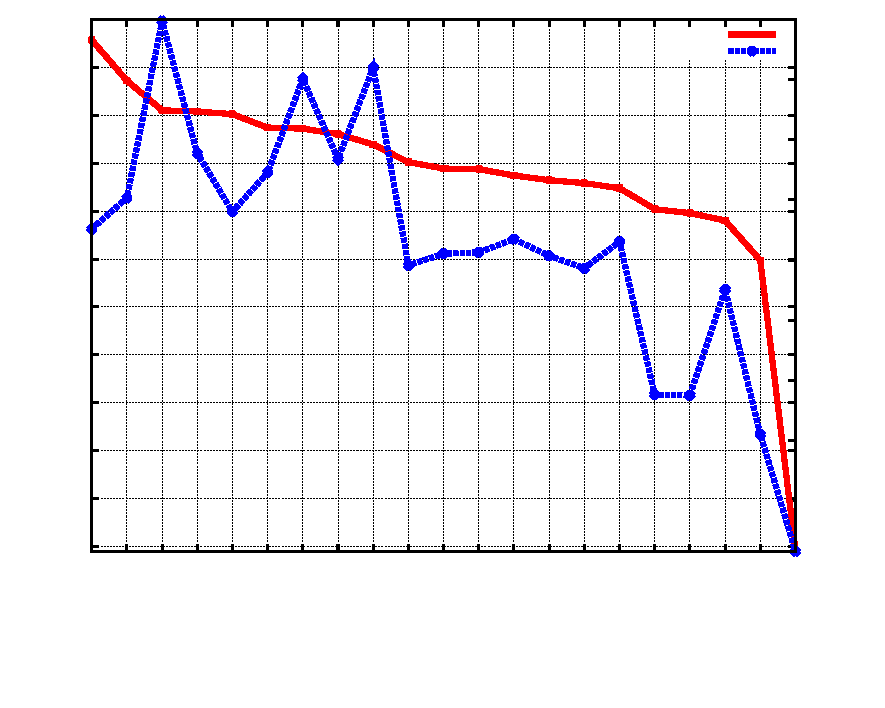
\includegraphics{plots/doc-X.pdf}}%
    \gplfronttext
  \end{picture}%
\endgroup
}
\caption{Doc classification.}
\label{fig:doc}
\end{figure}

\subsection{RNN \& Sequence Tagging}
\paragraph{Model}






\section{Analysis \& Discussion}\label{sec:analysis}
%SeqTag has much deeper networks than SentClass (and DocClass). But this has probably only effect when the task has long-range dependencies. [For doc class and sent class choice of activation function didn't matter much]
\paragraph{Winner statistics} 
%As seen in \S\ref{sec:experiments}, 
Each of the three meta-tasks sentence classification, document classification, and sequence tagging was won, on average, by a member from the rectifier family, namely, \relu{} (2) and \elu{}, for \best{}. Also, in each case, \cube{} and \cosid{} were among the worst performing activation functions. The majority of newly proposed functions from \citet{Ramach:2018} ranked somewhere in the mid-field, with \swish{} and \minsin{} performing best in the \best{} category.
For the \avg{} category, we particulary had the maxout functions as well as \pentan{} and \mysin{} regularly as top performers. 
%That the 
%The rectifier family performed much worse here is also evidenced by the fact that the winners of \best{} sometimes perform very badly on other task types; 
%for example, \elu{}, the winner for document classification, performed second-to-worst in sentence classification and in the mid-field for sequence tagging. 
%In contrast, \pentan{} was also always in the top group even for \best{}. 

To get further insights, we computed a winner statistic across all 17 mini-experiments, counting how often each activation function was among the top 3. Table \ref{table:topN} shows the results, excluding \prelu{} and the maxout functions because they were not considered in all mini-experiments. 

\begin{table}[!htb]
  \centering
  \begin{tabular}{ll}
  \toprule
     %         & Avg & Best \\ \midrule
    \best{} & \pentan{} (6), \swish{} (6), \\
    & \elu{} (4), \relu{} (4), \lrelua{} (4)\\   
    \avg{} & \pentan{} (16), \mytanh{} (13)\\
    & \mysin{} (10) \\
  \bottomrule
  \end{tabular}
  \caption{Top-3 winner statistics. In brackets: number of times within top-3, keeping only functions with four or more top-3 rankings.}
  \label{table:topN}
\end{table}

We see that \pentan{} and \swish{} win here for \best, followed by further rectifier functions. The \avg{} category is clearly won by saturating activation functions with finite range. If this comparison were restricted to sentence and document classification, where we also included the maxout functions, then \pentan{} would have been outperformed by maxout for \avg{}.

This appears to yield the conclusion that functions with limited range behave more stably across hyperparameter settings while non-saturating functions tend to yield better top-performances. The noteworthy exception to this rule is \pentan{} which excels in both categories (the more expensive maxout functions would be further exceptions). If the slope around the origin of \pentan{} is responsible for its good performance, then this could also explain why \cube{} is so bad, since it is very flat close to the origin.  

\paragraph{Influence of hyperparameters} To get some intuition about how hyperparameters affect our different activation functions, we regressed the score of the functions on the test set on all the employed hyperparameters. For example, we estimated:
\begin{align}\label{eq:regression}
  y = \alpha_l\cdot\log(n_l)+\alpha_d\cdot d+\cdots
\end{align}
where $y$ is the score on the test set, $n_l$ is the number of layers in the network, $d$ is the dropout value, etc. The coefficients $\alpha_k$ for each regressor $k$ is what we want to estimate (in particular, their size and their sign). We logarithmized certain variables whose scale was substantially larger than those of others (e.g., number of units, number of filters). For discrete regressors such as the optimizer we used binary dummy variables. We estimated Eq.~\eqref{eq:regression} independently for each activation function and for each mini-experiment. Overall, there was a very diverse pattern of outcomes, preventing us from making too strong conclusions. Still, we observed that while all models performed on average better with fewer hidden layers, particularly \swish{} was robust to more hidden layers (small negative coefficient $\alpha_l$), but also, to a lesser degree, \pentan{}. In the sentence classification tasks, \mysin{} and the maxout functions were particulary robust to an increase of hidden layers. Since \pentan{} is a saturating function and \mysin{} even an oscillating one, we therefore conclude that preserving the gradient (derivative close to one) is not a necessary prerequisite to successful learning in deeper neural networks. 



%\section{Related Work}\label{sec:related}

%\section{Problems}
%\subsection{Size matters}
People compare sentence embeddings of different sizes, but at the same time state that the evaluation measure, log.reg., performs better with higher-dimensional inputs.

\textbf{TODO}: evaluate 100,200,...,2000 dimensional word2vec embeddings.

\subsection{Comparing the uncomparable}
Citing numbers from previous papers which evaluated differently makes no sense.

\textbf{TODO}: Give numbers from sent2vec paper and our own evaluation of the method \todo{AR: we could even compare senteval, our own framework, and their values.}

\subsection{Which Classifier to use?}
Most researchers feed in to log.reg., some others feed sentence embeddings to deep averaging networks and CNNs (google paper). This makes things very uncomparable. The questions that arises is among others: is log.reg.\ eval justified when the embeddings would subsequently be used with more powerful networks anyway?

\textbf{TODO}: eval google embeddings in our own framework and perform some correlation analyses between log.reg.\ and CNN or deep average networks.

\todo{AR: Maybe even: Evaluate infersent with deep network, our own method with deep network. compare. We can also show how the effect is xling. do we get a bigger drop then with deep averaging, CNN? not suitable in many scenarios then.}

\subsection{Using cosine and Pearson correlation for evaluation of embeddings}
Problems: cosine and Pearson are arbitrary choices. Cosine/Pearson are not robust against certain normalizations. These kinds of evaluations may therefore be misleading. Better: learn the embedding function. Moreover: the google guys propose a variant of cosine because it ``performed better'' \todo{We need to propose solutions for being accepted. Learning sim could be one of them.}

\textbf{TODO}: make an experiment with learned embedding function vs.\ cosine and the cosine variant suggested in the google paper. Use concatenated p-means as an illustration.

\subsection{Several simple sentence embeddings techniques perform quite badly}
They even underperform word2vec\todo{Glove trained on huge huge corpus, not word2vec} embeddings. Problems: sent2vec, SIF, Siamese CBOW were all either evaluated for cosine or compared to very bad, and arbitrary, reference points (sent2vec). \todo{AR: Well, some methods might serve a purpose: retrieval. but I show that sent2vec for example is crap in retrieval. SIF might be better.}

\subsection{Using GPU vs.\ CPU}
Well, that's a minor point \todo{AR: This is mostly comparing liblinear against pytorch logreg implementation. Not GPU vs CPU actually. So it depends on how you implement logreg, actually.}

\subsection{The universal tasks are not universal}
For some the majority baseline is quite high. They're all on sentiment. \todo{AR: Yeah, but there is also this COCO retrieval stuff and semantic similarity we ignored due to weird evaluation}

\subsection{Hyper-Parameter tuning of log.reg.}
Optimizing learning rate may be crucial? \todo{AR: I would rather say: if you dont do hyperparam optimization properly you will get results that are worse than with proper hyperparams PER EMBEDDING TYPE.}

\subsection{Embeddings are trained on different data}
But people make claims about the techniques (glove better than word2vec), which is something to keep in mind. \todo{AR: Yes its all about the training data. Similar to NMT. But people already know this I guess?}



\section{Concluding remarks}\label{sec:conclusion}
%Which one should we use?
%
%Empirical comparison of rectifiers \cite{Xu:2015}
We have conducted the first large scale comparison of activation functions across several different NLP tasks (and task types) and using different popular neural network types. 
%To do so, we ran roughly X00K experiments. 
Our main focus was on so-called scalar activation functions, but we also partly included the more costly `many-to-one' %activation functions such as 
maxout functions. 
%that have higher resource demands. 

Our findings suggest that the rectifier functions (and the similarly shaped \swish{}) can be top performers for each task, but their performance is unstable and cannot be predicted a priori. One of our major findings is that, in contrast, the saturating \pentan{} function performs much more stably in this respect and can with high probability be expected to perform well across tasks as well as different choices of hyperparameters. This appears to make it the method of choice particularly when hyperparameter optimization is costly. When hyperparameter optimization is cheap, we recommend to consider the activation function as another hyperparameter and choose it, e.g., from the range of functions listed in Table \ref{table:topN} along with maxout. 

Another major advantage of the \pentan{} function is that it may also take the role of a gate (because of its finite range) and thus be employed in more sophisticated neural network units such as LSTMs, where the rectifiers fail completely. In this context, we noticed that replacing \sigmoid{} and \mytanh{} in an LSTM cell with \pentan{} leads to a 2pp increase on a challenging NLP sequence tagging task. Exploring whether this holds across more NLP tasks should be scope for future work. Additionally, our research suggests it is worthwhile to further explore \pentan{}, an arguably marginally known activation function. For instance, other scaling factors than $0.25$ (default value from \citet{Xu:2016}) should be explored. Similarly as for \prelu{}, the scaling factor can also be made part of the optimization problem. 

Finally, we found that except for \swish{} none of the newly discovered activation functions found in \citet{Ramach:2018} made it in our top categories, suggesting that automatic search of activation functions should be made across multiple tasks in the future. 

\section*{Acknowledgments}
We thank Teresa B\"otschen, Nils Reimers and the anonymous reviewers for helpful comments.
This work has been supported by the
German Federal Ministry of Education and Research
(BMBF) under the promotional reference
01UG1816B (CEDIFOR).

\bibliography{emnlp2018-2}
\bibliographystyle{acl_natbib}

%\section*{Appendix}
\appendix
\clearpage

%\newpage

\section{Supplemental Material}
Figures \ref{fig:saturating} and \ref{fig:nonsaturating} graph the 21 activation functions investigated in this paper.

\begin{figure}[!htb]
\scalebox{0.5}{
% GNUPLOT: LaTeX picture with Postscript
\begingroup
  \makeatletter
  \providecommand\color[2][]{%
    \GenericError{(gnuplot) \space\space\space\@spaces}{%
      Package color not loaded in conjunction with
      terminal option `colourtext'%
    }{See the gnuplot documentation for explanation.%
    }{Either use 'blacktext' in gnuplot or load the package
      color.sty in LaTeX.}%
    \renewcommand\color[2][]{}%
  }%
  \providecommand\includegraphics[2][]{%
    \GenericError{(gnuplot) \space\space\space\@spaces}{%
      Package graphicx or graphics not loaded%
    }{See the gnuplot documentation for explanation.%
    }{The gnuplot epslatex terminal needs graphicx.sty or graphics.sty.}%
    \renewcommand\includegraphics[2][]{}%
  }%
  \providecommand\rotatebox[2]{#2}%
  \@ifundefined{ifGPcolor}{%
    \newif\ifGPcolor
    \GPcolortrue
  }{}%
  \@ifundefined{ifGPblacktext}{%
    \newif\ifGPblacktext
    \GPblacktexttrue
  }{}%
  % define a \g@addto@macro without @ in the name:
  \let\gplgaddtomacro\g@addto@macro
  % define empty templates for all commands taking text:
  \gdef\gplbacktext{}%
  \gdef\gplfronttext{}%
  \makeatother
  \ifGPblacktext
    % no textcolor at all
    \def\colorrgb#1{}%
    \def\colorgray#1{}%
  \else
    % gray or color?
    \ifGPcolor
      \def\colorrgb#1{\color[rgb]{#1}}%
      \def\colorgray#1{\color[gray]{#1}}%
      \expandafter\def\csname LTw\endcsname{\color{white}}%
      \expandafter\def\csname LTb\endcsname{\color{black}}%
      \expandafter\def\csname LTa\endcsname{\color{black}}%
      \expandafter\def\csname LT0\endcsname{\color[rgb]{1,0,0}}%
      \expandafter\def\csname LT1\endcsname{\color[rgb]{0,1,0}}%
      \expandafter\def\csname LT2\endcsname{\color[rgb]{0,0,1}}%
      \expandafter\def\csname LT3\endcsname{\color[rgb]{1,0,1}}%
      \expandafter\def\csname LT4\endcsname{\color[rgb]{0,1,1}}%
      \expandafter\def\csname LT5\endcsname{\color[rgb]{1,1,0}}%
      \expandafter\def\csname LT6\endcsname{\color[rgb]{0,0,0}}%
      \expandafter\def\csname LT7\endcsname{\color[rgb]{1,0.3,0}}%
      \expandafter\def\csname LT8\endcsname{\color[rgb]{0.5,0.5,0.5}}%
    \else
      % gray
      \def\colorrgb#1{\color{black}}%
      \def\colorgray#1{\color[gray]{#1}}%
      \expandafter\def\csname LTw\endcsname{\color{white}}%
      \expandafter\def\csname LTb\endcsname{\color{black}}%
      \expandafter\def\csname LTa\endcsname{\color{black}}%
      \expandafter\def\csname LT0\endcsname{\color{black}}%
      \expandafter\def\csname LT1\endcsname{\color{black}}%
      \expandafter\def\csname LT2\endcsname{\color{black}}%
      \expandafter\def\csname LT3\endcsname{\color{black}}%
      \expandafter\def\csname LT4\endcsname{\color{black}}%
      \expandafter\def\csname LT5\endcsname{\color{black}}%
      \expandafter\def\csname LT6\endcsname{\color{black}}%
      \expandafter\def\csname LT7\endcsname{\color{black}}%
      \expandafter\def\csname LT8\endcsname{\color{black}}%
    \fi
  \fi
  \setlength{\unitlength}{0.0500bp}%
  \begin{picture}(8502.00,6802.00)%
    \gplgaddtomacro\gplbacktext{%
      \csname LTb\endcsname%
      \put(528,320){\makebox(0,0)[r]{\strut{}-1}}%
      \csname LTb\endcsname%
      \put(528,949){\makebox(0,0)[r]{\strut{}-0.8}}%
      \csname LTb\endcsname%
      \put(528,1578){\makebox(0,0)[r]{\strut{}-0.6}}%
      \csname LTb\endcsname%
      \put(528,2207){\makebox(0,0)[r]{\strut{}-0.4}}%
      \csname LTb\endcsname%
      \put(528,2836){\makebox(0,0)[r]{\strut{}-0.2}}%
      \csname LTb\endcsname%
      \put(528,3465){\makebox(0,0)[r]{\strut{} 0}}%
      \csname LTb\endcsname%
      \put(528,4093){\makebox(0,0)[r]{\strut{} 0.2}}%
      \csname LTb\endcsname%
      \put(528,4722){\makebox(0,0)[r]{\strut{} 0.4}}%
      \csname LTb\endcsname%
      \put(528,5351){\makebox(0,0)[r]{\strut{} 0.6}}%
      \csname LTb\endcsname%
      \put(528,5980){\makebox(0,0)[r]{\strut{} 0.8}}%
      \csname LTb\endcsname%
      \put(528,6609){\makebox(0,0)[r]{\strut{} 1}}%
      \csname LTb\endcsname%
      \put(624,160){\makebox(0,0){\strut{}-4}}%
      \csname LTb\endcsname%
      \put(1573,160){\makebox(0,0){\strut{}-3}}%
      \csname LTb\endcsname%
      \put(2521,160){\makebox(0,0){\strut{}-2}}%
      \csname LTb\endcsname%
      \put(3470,160){\makebox(0,0){\strut{}-1}}%
      \csname LTb\endcsname%
      \put(4419,160){\makebox(0,0){\strut{} 0}}%
      \csname LTb\endcsname%
      \put(5367,160){\makebox(0,0){\strut{} 1}}%
      \csname LTb\endcsname%
      \put(6316,160){\makebox(0,0){\strut{} 2}}%
      \csname LTb\endcsname%
      \put(7264,160){\makebox(0,0){\strut{} 3}}%
      \csname LTb\endcsname%
      \put(8213,160){\makebox(0,0){\strut{} 4}}%
    }%
    \gplgaddtomacro\gplfronttext{%
      \csname LTb\endcsname%
      \put(7478,943){\makebox(0,0)[r]{\strut{}\sigmoid(x)}}%
      \csname LTb\endcsname%
      \put(7478,783){\makebox(0,0)[r]{\strut{}\pentan(x)}}%
      \csname LTb\endcsname%
      \put(7478,623){\makebox(0,0)[r]{\strut{}\mytanh(x)}}%
      \csname LTb\endcsname%
      \put(7478,463){\makebox(0,0)[r]{\strut{}\mysin(x)}}%
    }%
    \gplbacktext
    \put(0,0){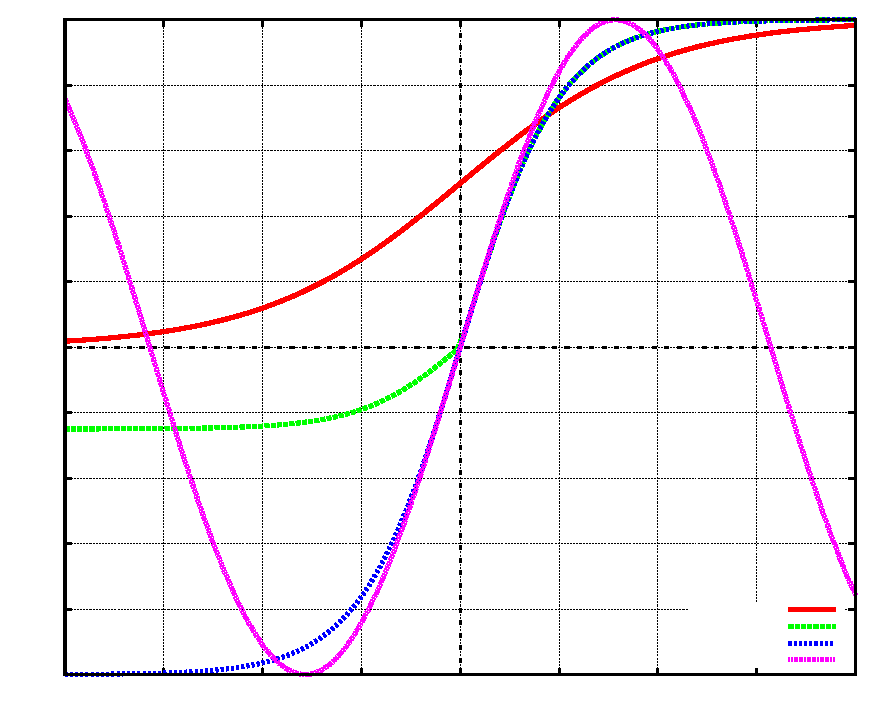
\includegraphics{plots/saturating-X.pdf}}%
    \gplfronttext
  \end{picture}%
\endgroup
}
\scalebox{0.5}{
% GNUPLOT: LaTeX picture with Postscript
\begingroup
  \makeatletter
  \providecommand\color[2][]{%
    \GenericError{(gnuplot) \space\space\space\@spaces}{%
      Package color not loaded in conjunction with
      terminal option `colourtext'%
    }{See the gnuplot documentation for explanation.%
    }{Either use 'blacktext' in gnuplot or load the package
      color.sty in LaTeX.}%
    \renewcommand\color[2][]{}%
  }%
  \providecommand\includegraphics[2][]{%
    \GenericError{(gnuplot) \space\space\space\@spaces}{%
      Package graphicx or graphics not loaded%
    }{See the gnuplot documentation for explanation.%
    }{The gnuplot epslatex terminal needs graphicx.sty or graphics.sty.}%
    \renewcommand\includegraphics[2][]{}%
  }%
  \providecommand\rotatebox[2]{#2}%
  \@ifundefined{ifGPcolor}{%
    \newif\ifGPcolor
    \GPcolortrue
  }{}%
  \@ifundefined{ifGPblacktext}{%
    \newif\ifGPblacktext
    \GPblacktexttrue
  }{}%
  % define a \g@addto@macro without @ in the name:
  \let\gplgaddtomacro\g@addto@macro
  % define empty templates for all commands taking text:
  \gdef\gplbacktext{}%
  \gdef\gplfronttext{}%
  \makeatother
  \ifGPblacktext
    % no textcolor at all
    \def\colorrgb#1{}%
    \def\colorgray#1{}%
  \else
    % gray or color?
    \ifGPcolor
      \def\colorrgb#1{\color[rgb]{#1}}%
      \def\colorgray#1{\color[gray]{#1}}%
      \expandafter\def\csname LTw\endcsname{\color{white}}%
      \expandafter\def\csname LTb\endcsname{\color{black}}%
      \expandafter\def\csname LTa\endcsname{\color{black}}%
      \expandafter\def\csname LT0\endcsname{\color[rgb]{1,0,0}}%
      \expandafter\def\csname LT1\endcsname{\color[rgb]{0,1,0}}%
      \expandafter\def\csname LT2\endcsname{\color[rgb]{0,0,1}}%
      \expandafter\def\csname LT3\endcsname{\color[rgb]{1,0,1}}%
      \expandafter\def\csname LT4\endcsname{\color[rgb]{0,1,1}}%
      \expandafter\def\csname LT5\endcsname{\color[rgb]{1,1,0}}%
      \expandafter\def\csname LT6\endcsname{\color[rgb]{0,0,0}}%
      \expandafter\def\csname LT7\endcsname{\color[rgb]{1,0.3,0}}%
      \expandafter\def\csname LT8\endcsname{\color[rgb]{0.5,0.5,0.5}}%
    \else
      % gray
      \def\colorrgb#1{\color{black}}%
      \def\colorgray#1{\color[gray]{#1}}%
      \expandafter\def\csname LTw\endcsname{\color{white}}%
      \expandafter\def\csname LTb\endcsname{\color{black}}%
      \expandafter\def\csname LTa\endcsname{\color{black}}%
      \expandafter\def\csname LT0\endcsname{\color{black}}%
      \expandafter\def\csname LT1\endcsname{\color{black}}%
      \expandafter\def\csname LT2\endcsname{\color{black}}%
      \expandafter\def\csname LT3\endcsname{\color{black}}%
      \expandafter\def\csname LT4\endcsname{\color{black}}%
      \expandafter\def\csname LT5\endcsname{\color{black}}%
      \expandafter\def\csname LT6\endcsname{\color{black}}%
      \expandafter\def\csname LT7\endcsname{\color{black}}%
      \expandafter\def\csname LT8\endcsname{\color{black}}%
    \fi
  \fi
  \setlength{\unitlength}{0.0500bp}%
  \begin{picture}(8502.00,6802.00)%
    \gplgaddtomacro\gplbacktext{%
      \csname LTb\endcsname%
      \put(336,320){\makebox(0,0)[r]{\strut{}-4}}%
      \csname LTb\endcsname%
      \put(336,1218){\makebox(0,0)[r]{\strut{}-3}}%
      \csname LTb\endcsname%
      \put(336,2117){\makebox(0,0)[r]{\strut{}-2}}%
      \csname LTb\endcsname%
      \put(336,3015){\makebox(0,0)[r]{\strut{}-1}}%
      \csname LTb\endcsname%
      \put(336,3914){\makebox(0,0)[r]{\strut{} 0}}%
      \csname LTb\endcsname%
      \put(336,4812){\makebox(0,0)[r]{\strut{} 1}}%
      \csname LTb\endcsname%
      \put(336,5711){\makebox(0,0)[r]{\strut{} 2}}%
      \csname LTb\endcsname%
      \put(336,6609){\makebox(0,0)[r]{\strut{} 3}}%
      \csname LTb\endcsname%
      \put(432,160){\makebox(0,0){\strut{}-3}}%
      \csname LTb\endcsname%
      \put(1729,160){\makebox(0,0){\strut{}-2}}%
      \csname LTb\endcsname%
      \put(3026,160){\makebox(0,0){\strut{}-1}}%
      \csname LTb\endcsname%
      \put(4323,160){\makebox(0,0){\strut{} 0}}%
      \csname LTb\endcsname%
      \put(5619,160){\makebox(0,0){\strut{} 1}}%
      \csname LTb\endcsname%
      \put(6916,160){\makebox(0,0){\strut{} 2}}%
      \csname LTb\endcsname%
      \put(8213,160){\makebox(0,0){\strut{} 3}}%
    }%
    \gplgaddtomacro\gplfronttext{%
      \csname LTb\endcsname%
      \put(7478,1103){\makebox(0,0)[r]{\strut{}\relu(x)}}%
      \csname LTb\endcsname%
      \put(7478,943){\makebox(0,0)[r]{\strut{}\swish(x)}}%
      \csname LTb\endcsname%
      \put(7478,783){\makebox(0,0)[r]{\strut{}\maxsig(x)}}%
      \csname LTb\endcsname%
      \put(7478,623){\makebox(0,0)[r]{\strut{}\cosid(x)}}%
      \csname LTb\endcsname%
      \put(7478,463){\makebox(0,0)[r]{\strut{}\minsin(x)}}%
    }%
    \gplbacktext
    \put(0,0){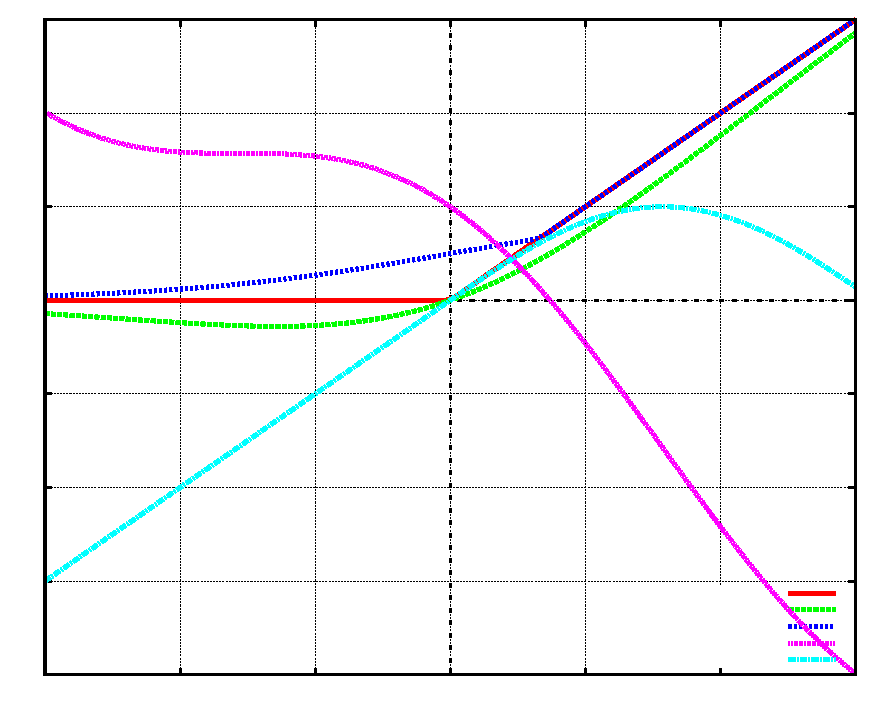
\includegraphics{plots/non-saturating1-X.pdf}}%
    \gplfronttext
  \end{picture}%
\endgroup

}
\caption{Several activation functions.}
\label{fig:saturating}
\end{figure}

\begin{figure}[!htb]
\scalebox{0.5}{
% GNUPLOT: LaTeX picture with Postscript
\begingroup
  \makeatletter
  \providecommand\color[2][]{%
    \GenericError{(gnuplot) \space\space\space\@spaces}{%
      Package color not loaded in conjunction with
      terminal option `colourtext'%
    }{See the gnuplot documentation for explanation.%
    }{Either use 'blacktext' in gnuplot or load the package
      color.sty in LaTeX.}%
    \renewcommand\color[2][]{}%
  }%
  \providecommand\includegraphics[2][]{%
    \GenericError{(gnuplot) \space\space\space\@spaces}{%
      Package graphicx or graphics not loaded%
    }{See the gnuplot documentation for explanation.%
    }{The gnuplot epslatex terminal needs graphicx.sty or graphics.sty.}%
    \renewcommand\includegraphics[2][]{}%
  }%
  \providecommand\rotatebox[2]{#2}%
  \@ifundefined{ifGPcolor}{%
    \newif\ifGPcolor
    \GPcolortrue
  }{}%
  \@ifundefined{ifGPblacktext}{%
    \newif\ifGPblacktext
    \GPblacktexttrue
  }{}%
  % define a \g@addto@macro without @ in the name:
  \let\gplgaddtomacro\g@addto@macro
  % define empty templates for all commands taking text:
  \gdef\gplbacktext{}%
  \gdef\gplfronttext{}%
  \makeatother
  \ifGPblacktext
    % no textcolor at all
    \def\colorrgb#1{}%
    \def\colorgray#1{}%
  \else
    % gray or color?
    \ifGPcolor
      \def\colorrgb#1{\color[rgb]{#1}}%
      \def\colorgray#1{\color[gray]{#1}}%
      \expandafter\def\csname LTw\endcsname{\color{white}}%
      \expandafter\def\csname LTb\endcsname{\color{black}}%
      \expandafter\def\csname LTa\endcsname{\color{black}}%
      \expandafter\def\csname LT0\endcsname{\color[rgb]{1,0,0}}%
      \expandafter\def\csname LT1\endcsname{\color[rgb]{0,1,0}}%
      \expandafter\def\csname LT2\endcsname{\color[rgb]{0,0,1}}%
      \expandafter\def\csname LT3\endcsname{\color[rgb]{1,0,1}}%
      \expandafter\def\csname LT4\endcsname{\color[rgb]{0,1,1}}%
      \expandafter\def\csname LT5\endcsname{\color[rgb]{1,1,0}}%
      \expandafter\def\csname LT6\endcsname{\color[rgb]{0,0,0}}%
      \expandafter\def\csname LT7\endcsname{\color[rgb]{1,0.3,0}}%
      \expandafter\def\csname LT8\endcsname{\color[rgb]{0.5,0.5,0.5}}%
    \else
      % gray
      \def\colorrgb#1{\color{black}}%
      \def\colorgray#1{\color[gray]{#1}}%
      \expandafter\def\csname LTw\endcsname{\color{white}}%
      \expandafter\def\csname LTb\endcsname{\color{black}}%
      \expandafter\def\csname LTa\endcsname{\color{black}}%
      \expandafter\def\csname LT0\endcsname{\color{black}}%
      \expandafter\def\csname LT1\endcsname{\color{black}}%
      \expandafter\def\csname LT2\endcsname{\color{black}}%
      \expandafter\def\csname LT3\endcsname{\color{black}}%
      \expandafter\def\csname LT4\endcsname{\color{black}}%
      \expandafter\def\csname LT5\endcsname{\color{black}}%
      \expandafter\def\csname LT6\endcsname{\color{black}}%
      \expandafter\def\csname LT7\endcsname{\color{black}}%
      \expandafter\def\csname LT8\endcsname{\color{black}}%
    \fi
  \fi
  \setlength{\unitlength}{0.0500bp}%
  \begin{picture}(8502.00,6802.00)%
    \gplgaddtomacro\gplbacktext{%
      \csname LTb\endcsname%
      \put(336,320){\makebox(0,0)[r]{\strut{}-2}}%
      \csname LTb\endcsname%
      \put(336,1218){\makebox(0,0)[r]{\strut{}-1}}%
      \csname LTb\endcsname%
      \put(336,2117){\makebox(0,0)[r]{\strut{} 0}}%
      \csname LTb\endcsname%
      \put(336,3015){\makebox(0,0)[r]{\strut{} 1}}%
      \csname LTb\endcsname%
      \put(336,3914){\makebox(0,0)[r]{\strut{} 2}}%
      \csname LTb\endcsname%
      \put(336,4812){\makebox(0,0)[r]{\strut{} 3}}%
      \csname LTb\endcsname%
      \put(336,5711){\makebox(0,0)[r]{\strut{} 4}}%
      \csname LTb\endcsname%
      \put(336,6609){\makebox(0,0)[r]{\strut{} 5}}%
      \csname LTb\endcsname%
      \put(432,160){\makebox(0,0){\strut{}-3}}%
      \csname LTb\endcsname%
      \put(1729,160){\makebox(0,0){\strut{}-2}}%
      \csname LTb\endcsname%
      \put(3026,160){\makebox(0,0){\strut{}-1}}%
      \csname LTb\endcsname%
      \put(4323,160){\makebox(0,0){\strut{} 0}}%
      \csname LTb\endcsname%
      \put(5619,160){\makebox(0,0){\strut{} 1}}%
      \csname LTb\endcsname%
      \put(6916,160){\makebox(0,0){\strut{} 2}}%
      \csname LTb\endcsname%
      \put(8213,160){\makebox(0,0){\strut{} 3}}%
    }%
    \gplgaddtomacro\gplfronttext{%
      \csname LTb\endcsname%
      \put(7478,1103){\makebox(0,0)[r]{\strut{}\arctid(x)}}%
      \csname LTb\endcsname%
      \put(7478,943){\makebox(0,0)[r]{\strut{}\maxtanh(x)}}%
      \csname LTb\endcsname%
      \put(7478,783){\makebox(0,0)[r]{\strut{}\lrelua(x)}}%
      \csname LTb\endcsname%
      \put(7478,623){\makebox(0,0)[r]{\strut{}\lrelub(x)}}%
      \csname LTb\endcsname%
      \put(7478,463){\makebox(0,0)[r]{\strut{}\elu(x)}}%
    }%
    \gplbacktext
    \put(0,0){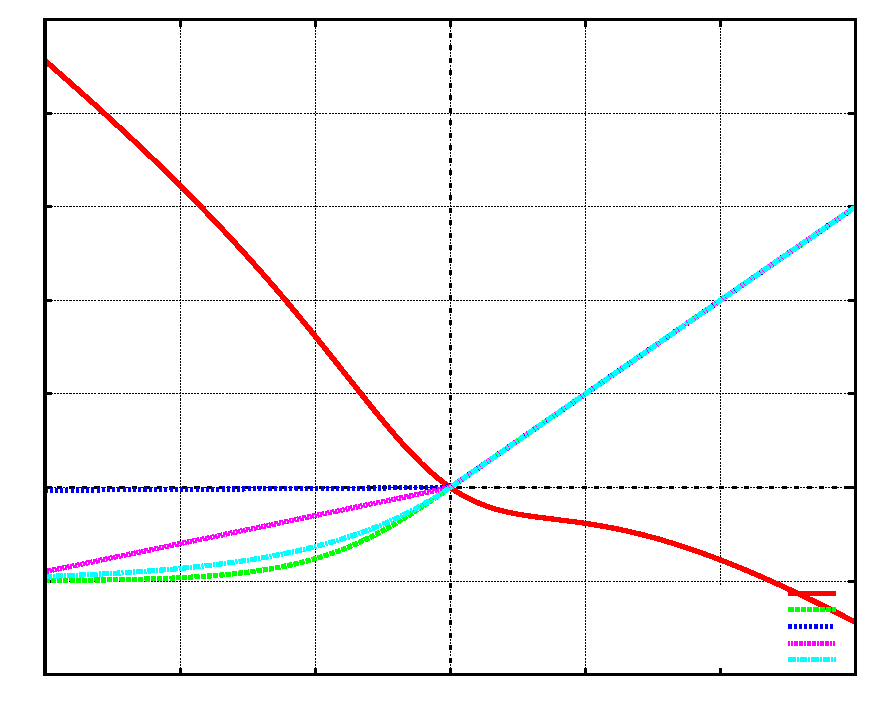
\includegraphics{plots/non-saturating2-X.pdf}}%
    \gplfronttext
  \end{picture}%
\endgroup
}
\scalebox{0.5}{
% GNUPLOT: LaTeX picture with Postscript
\begingroup
  \makeatletter
  \providecommand\color[2][]{%
    \GenericError{(gnuplot) \space\space\space\@spaces}{%
      Package color not loaded in conjunction with
      terminal option `colourtext'%
    }{See the gnuplot documentation for explanation.%
    }{Either use 'blacktext' in gnuplot or load the package
      color.sty in LaTeX.}%
    \renewcommand\color[2][]{}%
  }%
  \providecommand\includegraphics[2][]{%
    \GenericError{(gnuplot) \space\space\space\@spaces}{%
      Package graphicx or graphics not loaded%
    }{See the gnuplot documentation for explanation.%
    }{The gnuplot epslatex terminal needs graphicx.sty or graphics.sty.}%
    \renewcommand\includegraphics[2][]{}%
  }%
  \providecommand\rotatebox[2]{#2}%
  \@ifundefined{ifGPcolor}{%
    \newif\ifGPcolor
    \GPcolortrue
  }{}%
  \@ifundefined{ifGPblacktext}{%
    \newif\ifGPblacktext
    \GPblacktexttrue
  }{}%
  % define a \g@addto@macro without @ in the name:
  \let\gplgaddtomacro\g@addto@macro
  % define empty templates for all commands taking text:
  \gdef\gplbacktext{}%
  \gdef\gplfronttext{}%
  \makeatother
  \ifGPblacktext
    % no textcolor at all
    \def\colorrgb#1{}%
    \def\colorgray#1{}%
  \else
    % gray or color?
    \ifGPcolor
      \def\colorrgb#1{\color[rgb]{#1}}%
      \def\colorgray#1{\color[gray]{#1}}%
      \expandafter\def\csname LTw\endcsname{\color{white}}%
      \expandafter\def\csname LTb\endcsname{\color{black}}%
      \expandafter\def\csname LTa\endcsname{\color{black}}%
      \expandafter\def\csname LT0\endcsname{\color[rgb]{1,0,0}}%
      \expandafter\def\csname LT1\endcsname{\color[rgb]{0,1,0}}%
      \expandafter\def\csname LT2\endcsname{\color[rgb]{0,0,1}}%
      \expandafter\def\csname LT3\endcsname{\color[rgb]{1,0,1}}%
      \expandafter\def\csname LT4\endcsname{\color[rgb]{0,1,1}}%
      \expandafter\def\csname LT5\endcsname{\color[rgb]{1,1,0}}%
      \expandafter\def\csname LT6\endcsname{\color[rgb]{0,0,0}}%
      \expandafter\def\csname LT7\endcsname{\color[rgb]{1,0.3,0}}%
      \expandafter\def\csname LT8\endcsname{\color[rgb]{0.5,0.5,0.5}}%
    \else
      % gray
      \def\colorrgb#1{\color{black}}%
      \def\colorgray#1{\color[gray]{#1}}%
      \expandafter\def\csname LTw\endcsname{\color{white}}%
      \expandafter\def\csname LTb\endcsname{\color{black}}%
      \expandafter\def\csname LTa\endcsname{\color{black}}%
      \expandafter\def\csname LT0\endcsname{\color{black}}%
      \expandafter\def\csname LT1\endcsname{\color{black}}%
      \expandafter\def\csname LT2\endcsname{\color{black}}%
      \expandafter\def\csname LT3\endcsname{\color{black}}%
      \expandafter\def\csname LT4\endcsname{\color{black}}%
      \expandafter\def\csname LT5\endcsname{\color{black}}%
      \expandafter\def\csname LT6\endcsname{\color{black}}%
      \expandafter\def\csname LT7\endcsname{\color{black}}%
      \expandafter\def\csname LT8\endcsname{\color{black}}%
    \fi
  \fi
  \setlength{\unitlength}{0.0500bp}%
  \begin{picture}(8502.00,6802.00)%
    \gplgaddtomacro\gplbacktext{%
      \csname LTb\endcsname%
      \put(336,320){\makebox(0,0)[r]{\strut{}-3}}%
      \csname LTb\endcsname%
      \put(336,1218){\makebox(0,0)[r]{\strut{}-2}}%
      \csname LTb\endcsname%
      \put(336,2117){\makebox(0,0)[r]{\strut{}-1}}%
      \csname LTb\endcsname%
      \put(336,3015){\makebox(0,0)[r]{\strut{} 0}}%
      \csname LTb\endcsname%
      \put(336,3914){\makebox(0,0)[r]{\strut{} 1}}%
      \csname LTb\endcsname%
      \put(336,4812){\makebox(0,0)[r]{\strut{} 2}}%
      \csname LTb\endcsname%
      \put(336,5711){\makebox(0,0)[r]{\strut{} 3}}%
      \csname LTb\endcsname%
      \put(336,6609){\makebox(0,0)[r]{\strut{} 4}}%
      \csname LTb\endcsname%
      \put(432,160){\makebox(0,0){\strut{}-3}}%
      \csname LTb\endcsname%
      \put(1665,160){\makebox(0,0){\strut{}-2}}%
      \csname LTb\endcsname%
      \put(2898,160){\makebox(0,0){\strut{}-1}}%
      \csname LTb\endcsname%
      \put(4131,160){\makebox(0,0){\strut{} 0}}%
      \csname LTb\endcsname%
      \put(5363,160){\makebox(0,0){\strut{} 1}}%
      \csname LTb\endcsname%
      \put(6596,160){\makebox(0,0){\strut{} 2}}%
      \csname LTb\endcsname%
      \put(7829,160){\makebox(0,0){\strut{} 3}}%
      \put(7925,320){\makebox(0,0)[l]{\strut{}-3}}%
      \put(7925,1218){\makebox(0,0)[l]{\strut{}-2}}%
      \put(7925,2117){\makebox(0,0)[l]{\strut{}-1}}%
      \put(7925,3015){\makebox(0,0)[l]{\strut{} 0}}%
      \put(7925,3914){\makebox(0,0)[l]{\strut{} 1}}%
      \put(7925,4812){\makebox(0,0)[l]{\strut{} 2}}%
      \put(7925,5711){\makebox(0,0)[l]{\strut{} 3}}%
      \put(7925,6609){\makebox(0,0)[l]{\strut{} 4}}%
    }%
    \gplgaddtomacro\gplfronttext{%
      \csname LTb\endcsname%
      \put(7094,783){\makebox(0,0)[r]{\strut{}\selu(x)}}%
      \csname LTb\endcsname%
      \put(7094,623){\makebox(0,0)[r]{\strut{}\linear(x)}}%
      \csname LTb\endcsname%
      \put(7094,463){\makebox(0,0)[r]{\strut{}\cube(x)/10}}%
    }%
    \gplbacktext
    \put(0,0){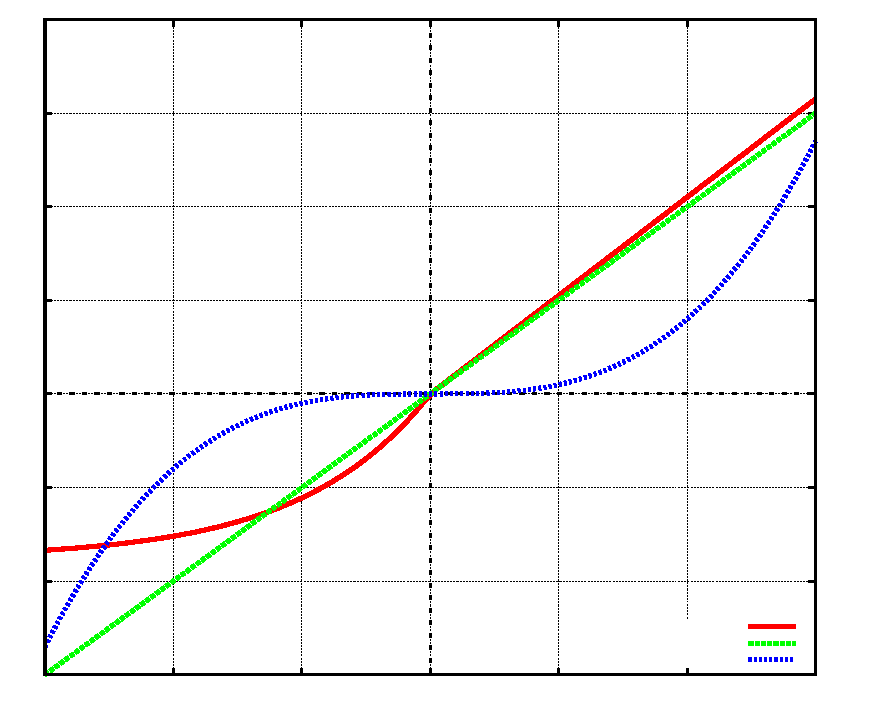
\includegraphics{plots/non-saturating3-X.pdf}}%
    \gplfronttext
  \end{picture}%
\endgroup

}
\caption{Several activation functions.}
\label{fig:nonsaturating}
\end{figure}


\end{document}
